\documentclass{izpit}
% Paket lahko naložite z neobveznimi možnostmi:
% - arhiv:
%     Izpis, namenjen za objavo izpita v arhivu. Naloge se pišejo ena pod
%     drugo, brez vmesnega prostora za reševanje, v glavi pa ni vpisnih polj.
% - izpolnjen:
%     Izpis, namenjen za generirane domače naloge. V glavi ni vpisnih polj,
%     saj se predpostavlja, da so že izpolnjena (vsak študent ima svojo
%     verzijo)
% - brezpaketov:
%     Prepreči nalaganje paketov amsmath, amssym, babel in inputenc. To
%     možnost uporabite, če je kakšen od teh paketov v konfliktu z vašimi.
%     Paketi ifthen, keyval, geometry in tikz se vedno naložijo, saj so
%     za uporabo paketa izpit obvezni.
% - sumniki:
%     Če vaš urejevalnik pod Windowsi ne pozna kodne tabele UTF-8
%     (ostali operacijski sistemi že leta podpirajo UTF-8),
%     uporabite možnost sumniki, da boste lahko pisali č namesto "c, ali \v c.
% - 10pt, 11pt, fleqn, ...
%     Uporabite lahko tudi vse ostale možnosti ki obstajajo v paketu article.
%     V osnovi je velikost črk 11pt.

\begin{document}

% Vsak izpit se začne z ukazom \izpit{predmet}{datum}{pravila}.
% Če želite v eni datoteki ustvariti več izpitov, lahko ukaz uporabite večkrat.
%
% Ukaz \izpit sprejme naslednje neobvezne možnosti:
% - ucilnica:
%     V glavo izpita se natisne shema učilnice, na kateri študentje lahko
%     označijo svoj sedež. Na voljo so učilnice: 201, 202, 203, 204, 205,
%     304, 305, 306, 307, 310, 311, 312, P01, P02, P04, P05, F1, F2, MFP in VFP.
%     Povejte, katere učilnice bi še potrebovali. Za idejo in pomoč pri izdelavi
%     se zahvaljujem Alešu Vavpetiču, Jaki Smrekarju in Janošu Vidaliju.
% - sedezni red:
%     Na shemi učilnice so dovoljeni sedeži odebeljeni.
% - naloge:
%     V glavo izpita se natisnejo okenca za vpis točk posameznih nalog ter
%     skupnega števila točk. Če je število nalog enako 0, se natisne samo
%     okence skupnega števila točk, če pa je negativno, se ne natisne nič. V
%     osnovi se natisnejo okenca za 4 naloge ter skupne točke.
% - anglescina:
%     Če želite izpit sestaviti v angleščini, uporabite parameter
%     'anglescina'. Prevedena bodo polja za ime, vpisno številko, oznake nalog
%     ter števila točk (če ste uporabili ukaz \tocke{} - glej spodaj).
% - nadaljuj:
%     Če izpit obsega več listov, lahko ukaz \izpit ponovimo na novem listu,
%     da se ponovno izpiše glava. Parameter 'nadaljuj' poskrbi za to, da se
%     števec nalog ne ponastavi in se tako številčenje nadaljuje na novem listu.
% - brez vpisne:
%     Polje za vnos vpisne številke se ne izriše.

\izpit[ucilnica = MFP, sedezni red, naloge = 3]
  {Diskretna algebraična analiza: 2. izpit}{11. 12. 2013}{
  Čas pisanja je 120 minut. Možno je doseči 100 točk. Veliko uspeha!
}

% Nalogo začnete z ukazom \naloga, podnalogo pa z ukazom \podnaloga. Oba ukaza
% sprejmeta neobvezen parameter, v katerega zapišete število točk.
% Na voljo vam je ukaz \tocke, ki sprejme število ter na konec doda besedo
% 'točke' (oz 'marks') s primerno končnico: \tocke{5} zapiše 5 točk,
% \tocke{102} zapiše 102 točki, ...
\naloga[\tocke{25}]

  \podnaloga[15]
    Poiščite izjavo $X = X(p, q, r)$, ki ima naslednjo pravilnostno tabelo.
    Izjavo poenostavite do oblike, ki vsebuje kvečjemu dva logična veznika.
    \[
      \begin{tabular}{c|cccccccc}
        $p$ & 1 & 1 & 1 & 1 & 0 & 0 & 0 & 0 \\
        $q$ & 1 & 1 & 0 & 0 & 1 & 1 & 0 & 0 \\
        $r$ & 1 & 0 & 1 & 0 & 1 & 0 & 1 & 0 \\\hline
        $X$ & 1 & 0 & 1 & 0 & 1 & 0 & 1 & 1 \\
      \end{tabular}
    \]
  
  % Ukaz \prostor na polo doda prostor za rešitev. Ukaz sprejme neobvezen
  % argument, ki pove, kolikšen delež prostora naj bo namenjen nalogi.
  % Če paket naložite z možnostjo 'arhiv', ukaz \prostor ne naredi ničesar.
  \prostor[2] % Za to nalogo bo dvakrat toliko prostora kot za naslednjo.

  \podnaloga[10]
    Naj bo $G$ grupa in $H$ njena podgrupa edinka. Dokažite, da grupa $G$ ni
    enostavna natanko tedaj, ko ima $H$ polbrata.

  \prostor

\naloga[\tocke{25}]
  Skicirajte graf funkcije $f \colon \mathbb{R} \to \mathbb{R}$, podane s
  predpisom
  \[
    f(x) = \frac{1 + x - x^2}{3 x^2 - 5} \;.
  \]

  % Ukaz \dodatek uporabite, kadar na izpit želite dati sliko, tabelo, ali kaj
  % podobnega, kar bo študentom v pomoč pri pisanju odgovorov.
  % Če paket naložite z možnostjo 'arhiv', ukaz \dodatek ne naredi ničesar.
  \dodatek{
    \[
      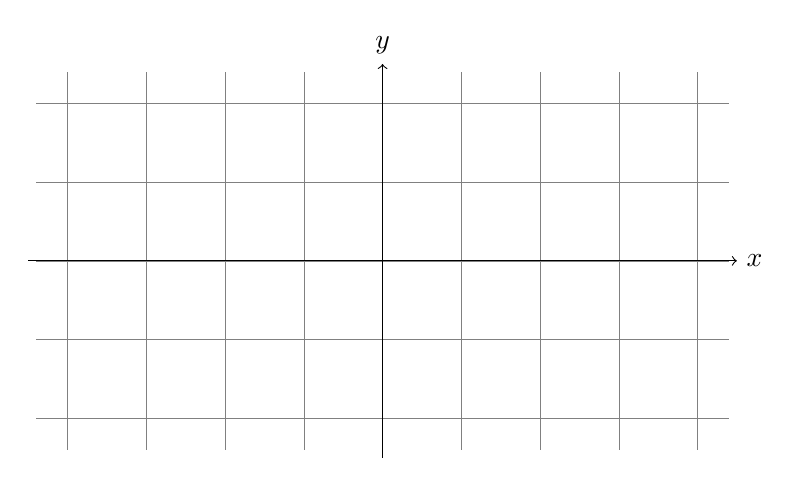
\begin{tikzpicture}
        \draw[help lines,step=1cm] (-4.4,-2.4) grid (4.4,2.4);
        \draw[->] (-4.5,0) -- (4.5,0) node[right] {$x$};
        \draw[->] (0,-2.5) -- (0,2.5) node[above] {$y$};
      \end{tikzpicture}
    \]
  }

% Vsaka naslednja naloga gre v osnovi na novo stran. Če želite nalogo dodati
% na isto stran, uporabite ukaz \naloga*, ki se obnaša enako kot \naloga, le
% da ne naredi nove strani.
\naloga*[brez točk]

  Za katera cela števila $c$ ima diofantska enačba
  \[
    72 x + 19 y = c
  \]
  rešitve v celih številih? Kakšna je v tem primeru splošna oblika rešitve?



\end{document}
